% 前言 (Introduction) --- 中译
% 原书 pp. xv--xix.

\chapter*{前言}
\markboth{前言}{前言}
\addcontentsline{toc}{chapter}{前言}

本书是一本适合高年级本科生或研究生初级阶段课程使用的代数导论.%
\index{daishu@代数}
尽管这一层次的教材选择极为丰富, 但在我讲授这些内容的过程中, 始终感到需要这样一本自成一体的书: 它``从零开始'' (即不假定读者此前对该学科已有大量接触), 却从一开始就贯彻相当现代的、以范畴%
\index{fanchou@范畴}
为纲的观点, 并力求达到相当的深度. 有许多代数教材出色地满足了其中部分、但并非全部的要求. 本书便是为提供一种切实可行的替代方案而作的一次尝试.

有一种流传甚广的观念认为, 初学时应当回避范畴, 认为范畴这种抽象语言要等到学生在数个学期的课程中通过以例子为主的方式领略了代数这类学科的品格之后, 才应当引入. 按照这种观点, 范畴与初等课程所涉及的主要课题只有边缘性的关联, 因而只需偶尔提及, 以泛泛地启发读者; 读者假以时日自会通晓它们 (靠潜移默化?). 套用本书草稿的一位审阅人的话说: ``在这一层次上讨论范畴, 正是上帝创造附录的原因.''

只要对目录稍加浏览便可看出, 我的想法并非如此. 在本书中, 范畴在第 $18$ 页即被引入, 此前只对朴素集合论%
\index{pusujihelun@朴素集合论}
的基本语言稍作回顾; 引入范畴的主要目的, 在于为万有性质%
\index{wanyouxingzhi@万有性质}
提供一个语境. 而在随后引入各种基本定义时, 又要不断诉诸万有性质. ``universal''这个词在前三章中至少出现了 $100$ 次.

我相信, 熟悉范畴语言---特别是对万有性质有所体会---对于``从一开始''就学习诸如代数这样的学科尤其有帮助. 我心目中的读者, 是已经具备一定程度数学成熟性的人---例如, 无需特别帮助便能理解一个归纳论证---但此前对代数可能只有非常粗浅的接触. 据我的经验, Florida State University 以及同类院校的许多高年级本科生和研究生低年级学生正符合这一描述. 对这些学生而言, 把代数中大量入门概念视为少数几个强有力的思想 (它们被封存在相应的万有性质之中) 的具体实例, 有助于为这些概念营建一个令人安心的统一语境. 起到这种催化作用所需的范畴语言其实非常有限; 例如, 在这个适应阶段其实并不真正需要函子%
\index{hanzi@函子}
.

因此, 在我看来, 这种做法的益处恰恰在于它能帮助真正的初学者---前提是使用得当. 这是我在课堂上的经验, 也是本书最主要的特色. 开篇引入的这一点点范畴语言贯穿了全书的第一部分, 以一般的方式引入群%
\index{qun@群}
、环%
\index{huan@环}
与模%
\index{mo@模}
. 随后是对若干标准课题的 (相当传统的) 处理, 诸如西罗%
\index{xiluo@西罗}
定理、唯一因子分解、初等线性代数与域论%
\index{yulun@域论}
. 全书的最后三分之一则涉入稍深的水域, 讨论张量积%
\index{zhangliangji@张量积}
与 Hom (包括对 Tor 与 Ext 的初步介绍), 并以专章同调代数%
\index{tongtiaodaishu@同调代数}
收尾. 在我看来, 若要领会这后一部分内容, 对范畴语言的某种程度的熟悉是不可或缺的; 这一点应该没有太大争议. 由于学生在本书前部已经对这种语言建立了感觉, 他们进入这些更深入的课题时会感到格外顺畅.

本书的第一个版本, 本质上是我在 FSU 一轮 (为期三学期的) 代数课程中讲稿的忠实誊录. 同调代数那一章是在 Ed Dunne 的怂恿下增补的, 习题中有相当大的一部分也是如此. 正文与最初的``讲稿''版本相比几乎没有变化: 在为出版而修订时, 我抵制了扩充材料的诱惑. 我认为, 一本有效的入门教材 (毕竟, 这是``第 $0$ 章''嘛\ldots) 应当是现实的: 书中所讲的内容必须能够在课堂上讲完. 否则, 本书就滑向了``参考书''一类; 我从未打算写一本代数参考书, 而且想要改进 Lang 的 \emph{Algebra}~\cite{lang2002algebra} 那样出色的现有参考书, 也注定是徒劳的.

这些习题集将为教师或任何有积极性的读者提供机会, 去触及比正文多得多的内容. 为便于挑选习题, 我用 $\triangleright$ 标记那些被正文直接引用的习题, 用 $\neg$ 标记那些被其他习题引用的习题. 一位极简主义的教师只需布置所有且仅有的 $\triangleright$ 习题即可; 这些习题不过是通过对练习来巩固理解, 对于一个既要承担助教工作、又要应付两三门与本课程强度相当的其他课程的学生而言, 它们大概就是其力所能及的全部. 正文连同这些习题, 构成了核心材料的一个自成一体的呈现. 其余的习题, 尤其是由 $\neg$ 标记的习题所勾画出的条条线索, 将提供覆盖其他课题的机会, 而其中一些课题完全可能被某些人视为同样不可或缺: 模群、四元数、幂零群、Artin 环、Jacobson 根、局部化、Lagrange 四平方定理、射影空间与 Grassmann 流形、Nakayama 引理、相伴素理想、正规算子的谱定理等等, 都是在习题中登场的课题的例子. 一个课题常常是跨越分布在书中适当位置的若干道习题逐步展开的. 例如, ``Wedderburn 小定理''在注记~III.1.16 中被提及 (即: 第三章的注记~1.16); 其特例出现在习题~III.2.11 与习题~IV.2.17 中, 而读者最终将在习题~VII.5.14 中得到它的一个证明, 其所需的预备内容则在习题~VII.5.12 与习题~VII.5.13 中给出. $\neg$ 标记连同对索引的查阅, 应当能为这类课题的导航提供便利. 为进一步助一臂之力, 我还为每道习题附上了 (加在方括号中的) 全书中引用它的位置清单. 例如, 一位正在考虑是否布置习题~V.2.25 的教师会立刻了解到: 这道题在习题~VII.5.18 中被引用, 后者证明了 Dirichlet 素数等差数列定理的一个特例, 而它又将在 \S VII.7.6 中被引用, 用以讨论把 Abel 群实现为 $\mathbb{Q}$ 上的 Galois 群.

我高度重视这样一项要求: 本书应当是自成一体的, 基本上把每个``t''都交叉、每个``i''都加点, 读者在研读本书时无需查阅其他书籍. 因此我有意识地努力不去引用其他文献: 我尽可能地避开那条诱人到极致的退路---``至于证明, 见\ldots''. 这正是本书之所以如此厚重的主要原因, 尽管书中还有如此多的课题未被涉及. 在这些缺席者中, 交换代数与表示论也许是最显眼的. 前者只以标准基本定义的程度出现, 这使我可以在这里或那里点缀一点代数几何 (例如见 \S VII.2), 并在习题中加入一些稍深入的课题, 但我止步于, 譬如说, 准素分解之前. 后者则完全没有涉及. 我希望在未来的某个 (尚未确定的) 时刻, 能以一个``第 $1$ 章''来补全本书, 届时我将为这些以及其他缺憾作出弥补.

本书的性质使它相当适合自学: 自学的读者将在本书中找到一个自成一体的起点, 它应当可以很好地充当未来更深入探索的序曲. 这样的读者也许会受益于下面这幅展示各章之间逻辑依赖关系的``九重之路''图:

\begin{figure}[ht]
	\centering
	\begin{tikzpicture}[box/.style={draw, semithick, minimum width=1.35cm, minimum height=0.85cm, font=\Large}, >=Stealth, semithick]
		\node[box] (I)   at (0.0, 0.0) {I};
		\node[box] (II)  at (2.1, 0.9) {II};
		\node[box] (III) at (2.1,-0.9) {III};
		\node[box] (IV)  at (4.0, 2.0) {IV};
		\node[box] (VII) at (4.2, 0.0) {VII};
		\node[box] (V)   at (4.4,-2.0) {V};
		\node[box] (VI)  at (6.6,-1.0) {VI};
		\node[box] (IX)  at (6.8, 1.2) {IX};
		\node[box] (VIII) at (9.0, 0.0) {VIII};
		\draw[->] (I) -- (II);
		\draw[->] (I) -- (III);
		\draw[->] (II) -- (III);
		\draw[->] (II) -- (IV);
		\draw[->] (II) -- (VII);
		\draw[->] (III) -- (V);
		\draw[->] (IV) -- (VII);
		\draw[->] (V) -- (VII);
		\draw[->] (V) -- (VI);
		\draw[->] (VI) -- (VII);
		\draw[->] (VI) -- (VIII);
		\draw[->] (VI) -- (IX);
		\draw[->] (VIII) -- (IX);
	\end{tikzpicture}
\end{figure}

不过, 这幅图更多地反映了我最初的意图, 而不是最终的产品. 作为一个更客观的尺度, 下面这幅替代性的图画出了各章对前面各章的引用之网, 线条的粗细大致代表引用次数的多少:

\begin{figure}[ht]
	\centering
	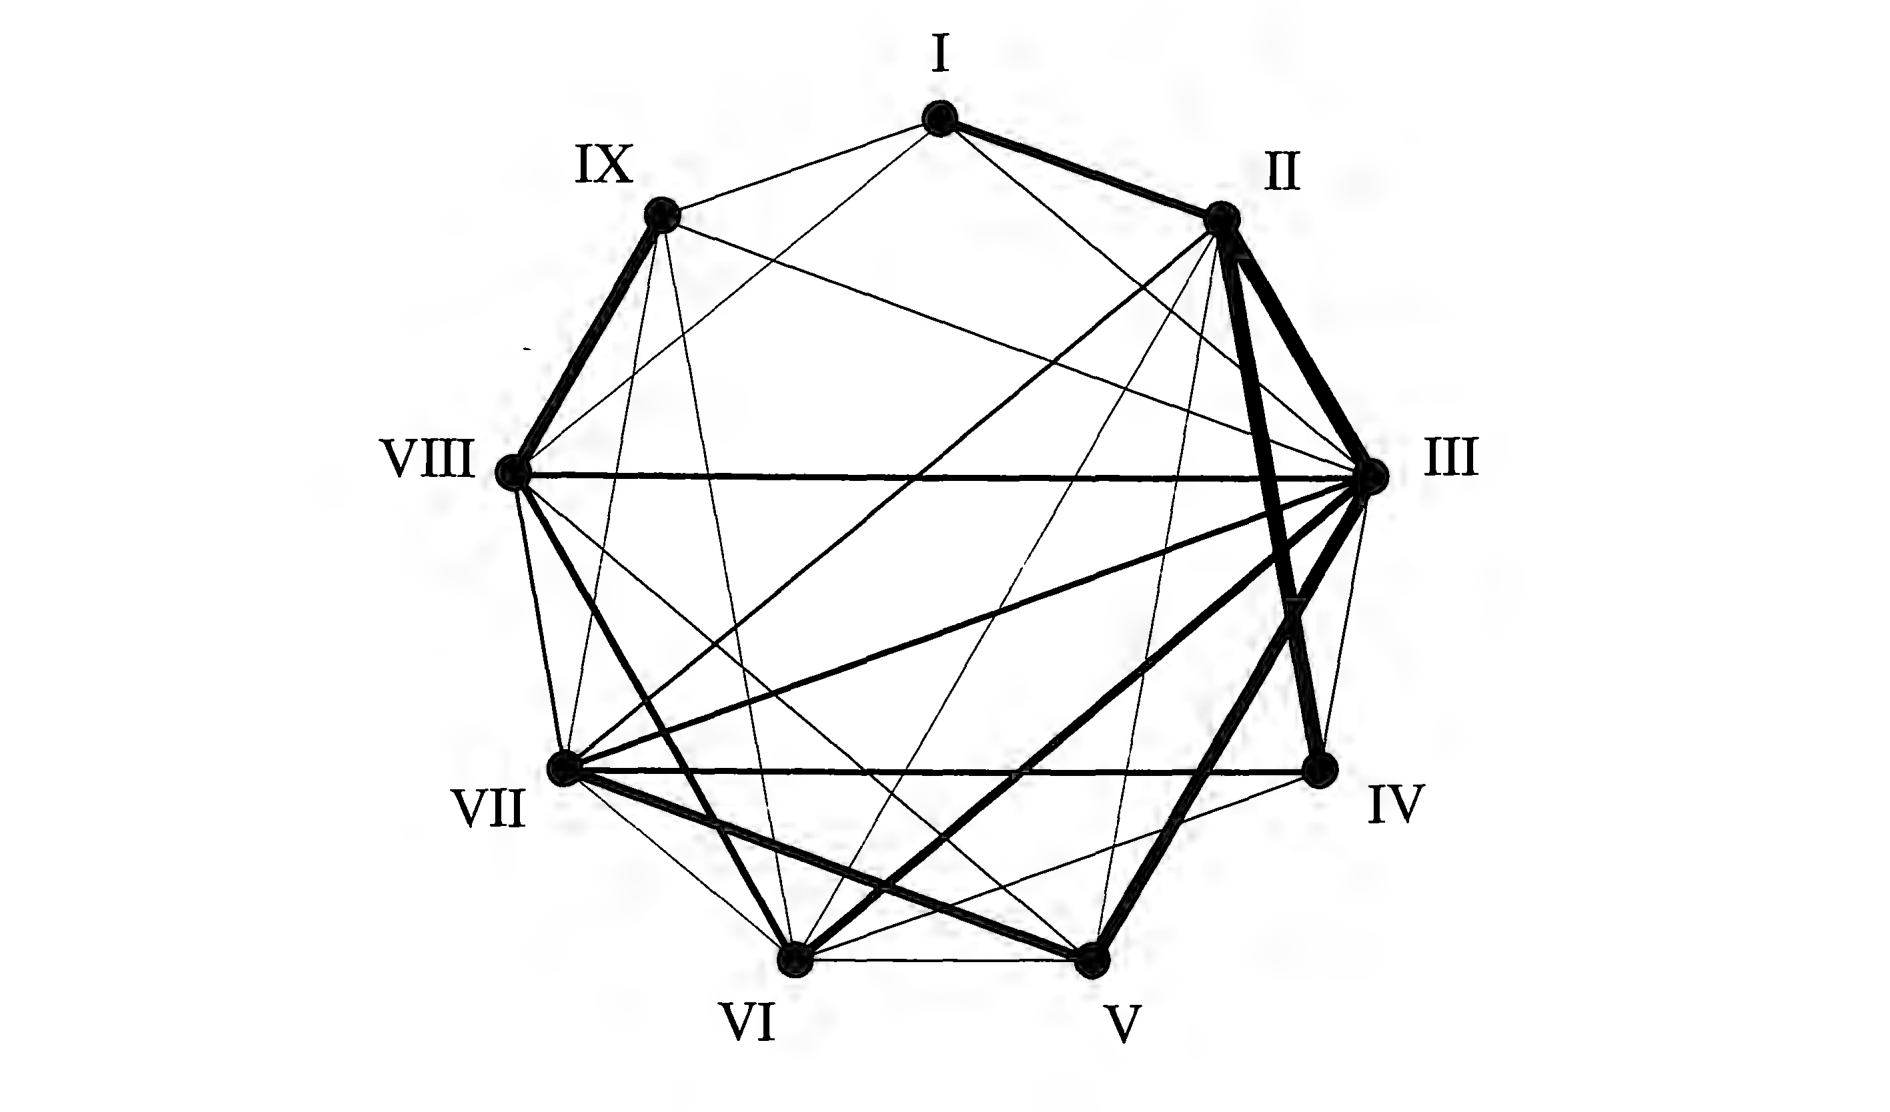
\includegraphics[width=0.62\textwidth]{figs/intro-web.png}
\end{figure}

我特别照顾到了自学的读者, 因而在编制详尽的索引上格外下了一番功夫. 对于一本书的这种篇幅, 不可能为引入的每一个新术语都安排一次正式的``定义''来大事张扬; 索引应当帮助独自旅行的读者找到陌生术语的源头.

书内交叉引用的处理方式希望是透明的. 例如, 注记~III.1.16 指第三章的注记~1.16; 若引用出自第三章内部, 则同一对象就称为注记~1.16. 习题后面方括号中的清单, 列出了书中引用该习题的其他习题或节. 例如, 第一章的习题~3.1 后面跟着 $[\,5.1,\ \S$VIII.1.1$,\ \S$IX.1.2$,\ \text{IX.1.10}\,]$: 这提醒读者, 本题在第一章的习题~5.1、第八章的 \S 1.1、第九章的 \S 1.2 以及第九章的习题~1.10 中被引用 (而且仅在这些地方).

\emph{致谢.} 我对 Lang 的教材~\cite{lang2002algebra}、David Dummit 与 Richard Foote 的 \emph{Abstract Algebra}~\cite{dummitfoote2004abstract} 以及 Michael Artin 的 \emph{Algebra}~\cite{artin1991algebra} 的亏欠, 凡熟悉这些书的人都不难看出. 同调代数那一章则很大程度上得益于 David Eisenbud 的 \emph{Commutative Algebra}~\cite{eisenbud1995commutative} 中论及该主题的附录、Gelfand--Manin 的 \emph{Methods of Homological Algebra}~\cite{gelfandmanin2003methods} 以及 Weibel 的 \emph{An Introduction to Homological Algebra}~\cite{weibel1994introduction}. 但在大多数情形下, 我实在无法追溯某个叙述性的想法、某个证明、某道习题或某种特定的教学侧重最初的来源: 它们多半是这些以及其他有影响的文献中思想的产物, 也常常源于在万维网的万千线索间穿行时触发的联想. 这也是为何我以一种心平气和的精神, 决定基本上完全不列参考文献的另一个原因. 无论如何, 我相信这里呈现的所有材料都是标准的; 对于成品中遗留下来的每一个错误, 我保留绝对的所有权.

我非常感谢我的学生们, 他们持续不断的反馈促使我以这种特定方式写作本书, 并为本书在我课堂上的成功作出了实质性的贡献. 一些学生向我提供了长长的排印错误乃至不折不扣的错误的清单, 我要特别感谢 Kevin Meek、Jay Stryker 与 Yong Jae Cha 极有帮助的意见. $2008$ 年秋, 在 FSU 学术休假期间, 我有机会在 Caltech 的一门课程中试用同调代数的材料, 我感谢 Caltech 以及选课的听众们的热情接待与友好氛围. 也感谢 MSRI 在 $2009$ 年冬天提供的接待, 本书最后的打磨正是在那时完成的.

有几位同行在本书的预备版本中发现了大大小小的错误, 我要提到 Georges Elencwajg、Xia Liao 与 Mirroslav Yotov, 他们的贡献尤为宝贵. 我也要赞扬 Arlene O'Sean 与 AMS 的编辑制作团队出色的文字编辑与制作工作.

特别感谢 Ettore Aldrovandi 的专业建议、Matilde Marcolli 的鼓励与不可或缺的帮助, 以及 Ed Dunne 对本书最终版本的形成影响深远的诸多建议.

本书撰写各阶段所获的 Max-Planck-Institut (Bonn)、NSA 以及 Caltech 的支持, 在此一并致谢.
